%%%%%%%%%%%%%%%%%%%%%%%%%%%%%%%%%%%%%%%%%%%%%%%%%%%%%%%%%%%%%%%%%%%%%%%%%%%%%%%%
%2345678901234567890123456789012345678901234567890123456789012345678901234567890
%        1         2         3         4         5         6         7         8

\documentclass[letterpaper, 10 pt, conference]{ieeeconf}  % Comment this line out if you need a4paper
\usepackage[utf8]{inputenc}
\usepackage{graphicx}
\usepackage{amsmath}
\usepackage{hyperref}
\usepackage{cleveref}
\usepackage{amssymb}
\usepackage[table]{xcolor}% http://ctan.org/pkg/xcolor
\usepackage{xcolor}
\usepackage{epsfig}
\let\labelindent\relax
\usepackage{enumitem}
\usepackage{pgf,tikz}
\usetikzlibrary{decorations.pathreplacing,calligraphy}
\usepackage{makecell}
\usepackage{mdframed}% http://ctan.org/pkg/mdframed
%\usepackage{geometry}

%\documentclass[a4paper, 10pt, conference]{ieeeconf}      % Use this line for a4 paper

\IEEEoverridecommandlockouts                              % This command is only needed if 
% you want to use the \thanks command

\overrideIEEEmargins                                      % Needed to meet printer requirements.

%In case you encounter the following error:
%Error 1010 The PDF file may be corrupt (unable to open PDF file) OR
%Error 1000 An error occurred while parsing a contents stream. Unable to analyze the PDF file.
%This is a known problem with pdfLaTeX conversion filter. The file cannot be opened with acrobat reader
%Please use one of the alternatives below to circumvent this error by uncommenting one or the other
%\pdfobjcompresslevel=0
%\pdfminorversion=4

% See the \addtolength command later in the file to balance the column lengths
% on the last page of the document

% The following packages can be found on http:\\www.ctan.org
%\usepackage{graphics} % for pdf, bitmapped graphics files
%\usepackage{epsfig} % for postscript graphics files
%\usepackage{mathptmx} % assumes new font selection scheme installed
%\usepackage{times} % assumes new font selection scheme installed
%\usepackage{amsmath} % assumes amsmath package installed
%\usepackage{amssymb}  % assumes amsmath package installed

%\title{\LARGE \bf
%	JAEGO : Attention Sharing in Sensory Egocentric Spheres
%}
%\title{\LARGE \bf
%	From Egocentric Sensory Sphere to Joint Attention and Back 
%}
\title{\LARGE \bf
	JA-EGO : The Ego-sensory Sphere of Joint Attention
}


\author{Hendry Ferreira Chame$^{1}$ and Rachid Alami$^{2}$% <-this % stops a space
	%\thanks{*This work was not supported by any organization}% <-this % stops a space
	\thanks{$^{1}$Team NeuroRhythms at LORIA-CNRS, Campus Scientifique, 615 Rue du Jardin-Botanique, 54506 Vand\oe uvre-l\`es-Nancy, France.
		{\tt\small hendry.ferreira-chame@loria.fr}}%
	\thanks{$^{2}$Team Robotics and InteractionS (RIS) at LAAS-CNRS, Universit\'e de Toulouse, CNRS, Toulouse, France
		{\tt\small rachid.alami@laas.fr}}%
}


\begin{document}
		
	
	\maketitle
	\thispagestyle{empty}
	\pagestyle{empty}
	
	
	%%%%%%%%%%%%%%%%%%%%%%%%%%%%%%%%%%%%%%%%%%%%%%%%%%%%%%%%%%%%%%%%%%%%%%%%%%%%%%%%
	\begin{abstract}
		
		\small \bf In everyday life we frequently run into face-to-face interactions where we quickly share attention and communicate about objects with others, be it for providing guidance to someone or commenting or some unusual thing or event, to name a few examples. In such situations, we don’t think too much about it, although we may not necessarily know where we are, we can talk about things in the environment even when seeing for the first time. As addressed in Moravec's Paradox, for human-robot interaction research, the scenario is not as simple as for human interaction. However, progress has been achieved when departing from cognitivist philosophy and embracing embodiment and 4E cognition research, as a source of inspiration for designing light and efficient models of interaction. This work goes in this direction and proposes a sensory fusion mechanism named JAEGO relying mostly on immediate perception and low level cognitive skills such as working memory, so a robot is able to share attention with the human based on local (egocentric) sources of information and very simple proxemics. The advantage of our approach is that, by exploiting embodiment, a very efficient and intuitive communication system can result, which is adaptable to everyday situations not requiring the agent to process extensive information about the environment. In order to assess our hypothesis, we performed studies in simulation and a real interaction with the robot Pepper in a joint attention task. Results showed the robot is able to correctly focus on objects of interest in the environment when interacting with the human.   
		
	\end{abstract}
	
	
	%%%%%%%%%%%%%%%%%%%%%%%%%%%%%%%%%%%%%%%%%%%%%%%%%%%%%%%%%%%%%%%%%%%%%%%%%%%%%%%%
	\section{INTRODUCTION}
	
	This is the introduction of the research ...
	
	\section{RELATED WORK}
	%Biological studies have pointed out to the existence of biological mechanisms to support essential cognitive functions such as attention, short-term memory, spatio-temporal sensory-motor coordination, and locomotion, among others.

	Some works in the field of robotics have achieved impressive results by exploring attention saliency in sensory egocentric representations (e.g. for bottom-up \cite{ruesch2008} and top-down \cite{bodiroza2011} mechanisms). Most of these works have considered a sort of environment exploration task, so the robot can focus on learning new things based on novelty. Fewer research have studied joint attention tasks (e.g. \cite{bodiroza2011}) inspired on psychological theories of attention. Overall, the representation proposed has neglected bio-inspiration on neural systems, consisting mostly in storage arrays for data indexed by spherical tessellation mapping (see \cite{peters2009sensory}). As a result, the dynamics of pre-attentive processing has not being modeled as a process unfolding in the same space where attention selection is done. We believe that this is an important limitation, when considering the possibility of investigating compositionality in joint attention as a descending (top-down) generative process combined with an ascending (bottom-up) saliency process, susceptible of study as a dynamical system.   
	
	Another limitation of previous research is considering the robot as the only one in interaction given with embodied ego-sensory mapping representations, so data coming from the human is mostly represented in the robot ego-sensory sphere. In our opinion, this would be a too much egocentric view of joint action in HRI. Thus, the robot should be able to represent its own world while accepting the egocentric view of others and being able to handle such body correspondences dynamically. 
	 
	From our perspective, different works have constituted previous steps in the direction of proposing our current study which is worth mentioning. The work by \cite{chame2016} has proposed a sensory ego-cylindrical information fusion mechanism for egocentric localization allowing the robot to autonomous position with respect to object in the environment based on embodied representations. Concerning joint attention modeling, the model TOP-JAM \cite{chame2023top} was proposed for interaction situations mediated by objects where allocentric references for addressing the task would make sense (e.g. sharing attention around a table, participating in an assembly collaboration task, to name a few) considering an extended range of knowledge and attention sharing (i.e. individual, monitoring, common, and sharing \cite{siposova2019}). 
	 
	
	% 
	
	
	%More importantly, attention clues from the human are not processed in the same representation space
	
	%attention processes dynamics has not been 
	
	%the body posture of the human has not being considered as an source of information for the robot attention process. Moreover, the sensory ego-sphere has been proposed as a computational data structure which does not represents directly the focus of attention of participants, neglecting thus the dynamics of interaction, consisting mostly in a data storage repository indexed by tessellation spherical mapping (see \cite{peters2009sensory}). 
	
	
	
	
	%\cite{ruesch2008}
	
	%The problem of placement of the egocentric localization reference is not trivial and would greatly depend on the task at hand.   
	
	%The origin of the ego-cylinder can be fixed to different parts of the body. There is no agreement in the literature on the placement for this structure.
	
	
	 %... in the field of cognitive robotics, the work by \cite{peters2009sensory} has proposed a data structure in the form of a sensory ego-sphere located at the robot base frame as a mediating interface between sensors and cognitive processes. 
	 
	%The work by \cite{chame2016} has proposed a sensory ego-cylindrical information fusion mechanism for egocentric localization allowing the robot to autonomous position with respect to object in the environment based on embodied representations. 
	
	\begin{figure}[h!]
		\begin{center}
		\begin{tikzpicture}
		\node [] at (0,0){
			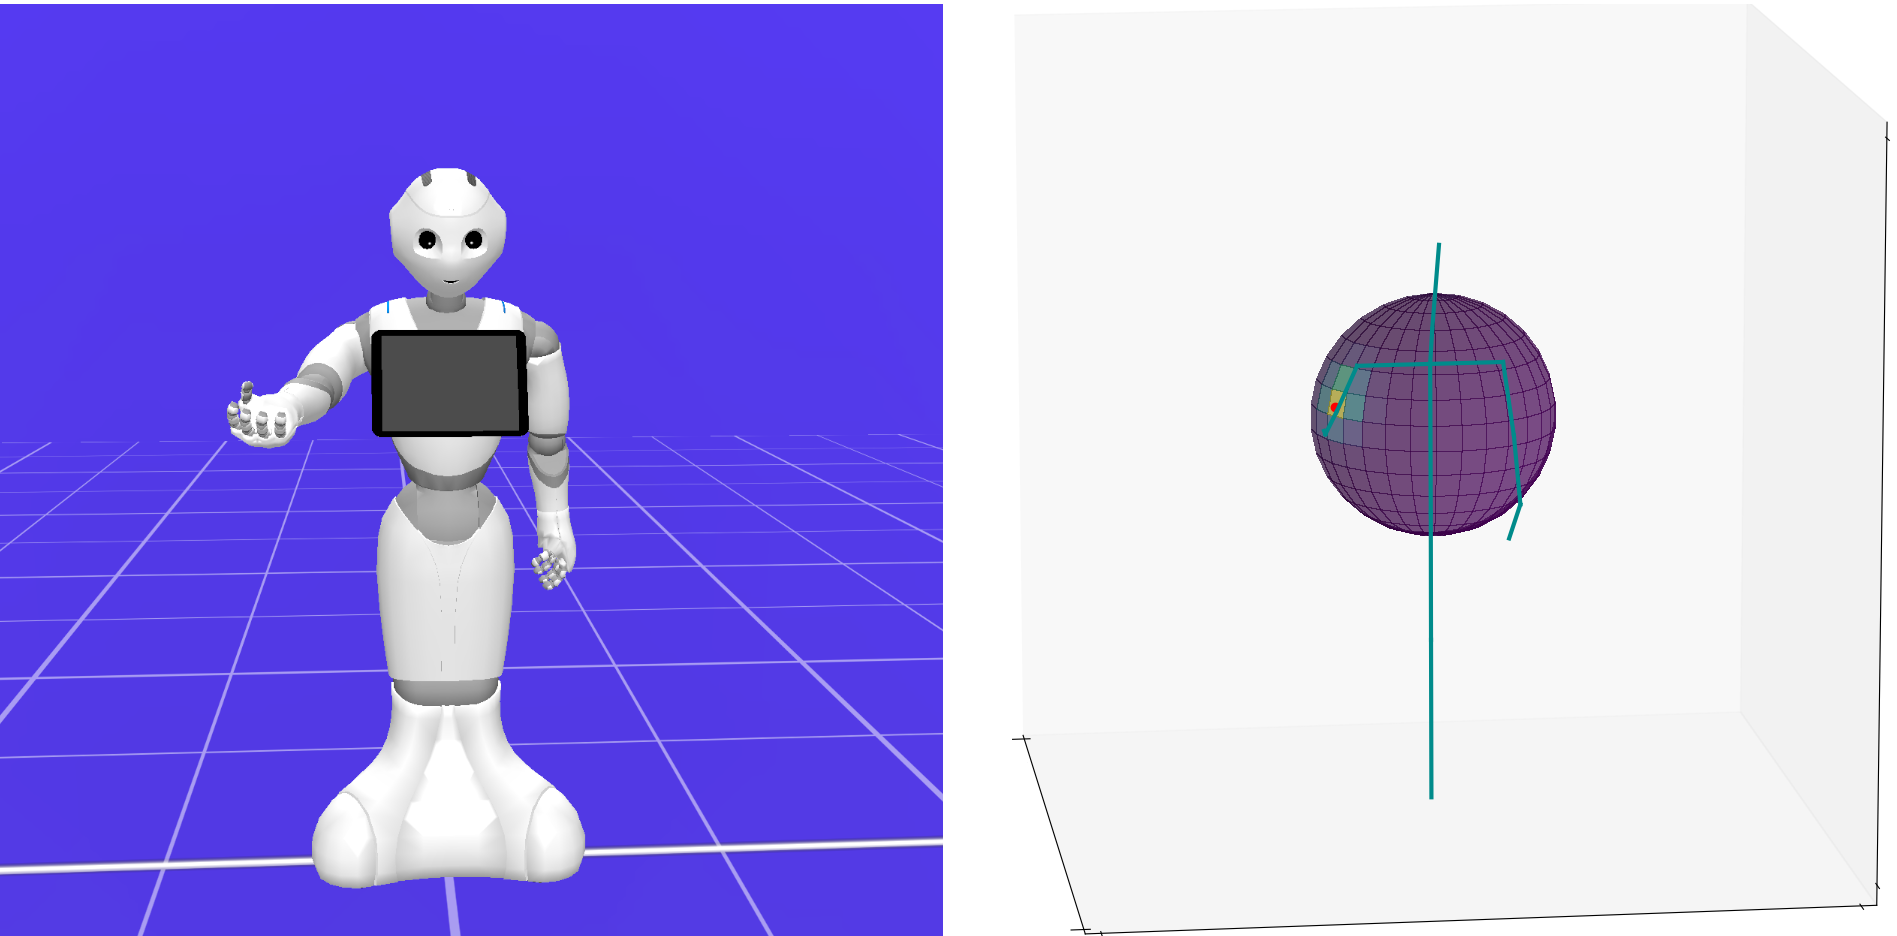
\includegraphics[scale=0.5,keepaspectratio]{fig/robot_pointing.png}};
		\node at (0.0,2.4) [color=black] {\small \textbf{The robot sensory ego-sphere}};
		\end{tikzpicture}
		\caption{Left: the robot is pointing to a location in the space. Right: the attention state of the robot is shown as the activation of the neural network representing the sensory ego-sphere, as stimulated by the intersection of the forearm direction with by the sensory ego-sphere.}
		\label{fig:robot_pointing}
		\end{center}
	\end{figure}

	
	\section{THE MATHEMATICAL MODEL}
	
	Let a ego-sphere representation of sensory information be modeled by the following neural network architecture \cite{amari1977}.
	
		\begin{figure}[h!]
		\begin{center}
			\begin{tikzpicture}
			\node [] at (0,0){
				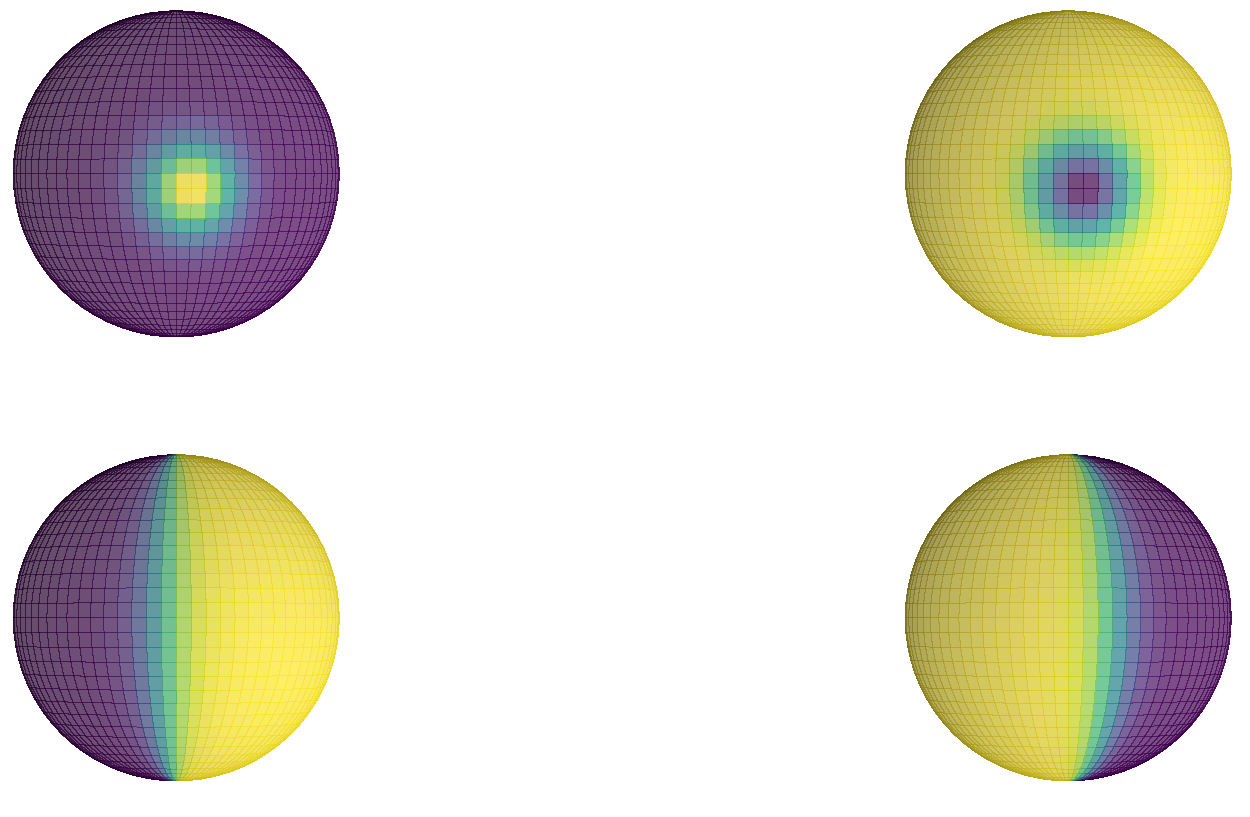
\includegraphics[scale=0.7,keepaspectratio]{fig/filters.png}};
			\node at (0.0,2.6) [color=black] {\small \textbf{Pre-selection filters}};
			\node at (-2.6,0.1) [color=black] {\scriptsize Point excitation};
			\node at (2.6,0.1) [color=black] {\scriptsize Point inhibition};
			\node at (-2.7,-2.4) [color=black] {\scriptsize Right-side excitation};
			\node at (2.7,-2.4) [color=black] {\scriptsize left-side excitation};
			
			\end{tikzpicture}
			\caption{Filters functions affecting the pre-selection phase.}
			\label{fig:filters}
		\end{center}
	\end{figure}
	
	\section{PROCEDURE FOR PAPER SUBMISSION}
	
	\subsection{Selecting a Template (Heading 2)}
	
	First, confirm that you have the correct template for your paper size. This template has been tailored for output on the US-letter paper size. 
	It may be used for A4 paper size if the paper size setting is suitably modified.
	
	\subsection{Maintaining the Integrity of the Specifications}
	
	The template is used to format your paper and style the text. All margins, column widths, line spaces, and text fonts are prescribed; please do not alter them. You may note peculiarities. For example, the head margin in this template measures proportionately more than is customary. This measurement and others are deliberate, using specifications that anticipate your paper as one part of the entire proceedings, and not as an independent document. Please do not revise any of the current designations
	
	\section{MATH}
	
	Before you begin to format your paper, first write and save the content as a separate text file. Keep your text and graphic files separate until after the text has been formatted and styled. Do not use hard tabs, and limit use of hard returns to only one return at the end of a paragraph. Do not add any kind of pagination anywhere in the paper. Do not number text heads-the template will do that for you.
	
	Finally, complete content and organizational editing before formatting. Please take note of the following items when proofreading spelling and grammar:
	
	\subsection{Abbreviations and Acronyms} Define abbreviations and acronyms the first time they are used in the text, even after they have been defined in the abstract. Abbreviations such as IEEE, SI, MKS, CGS, sc, dc, and rms do not have to be defined. Do not use abbreviations in the title or heads unless they are unavoidable.
	
	\subsection{Units}
	
	\begin{itemize}
		
		\item Use either SI (MKS) or CGS as primary units. (SI units are encouraged.) English units may be used as secondary units (in parentheses). An exception would be the use of English units as identifiers in trade, such as 03.5-inch disk drive.
		\item Avoid combining SI and CGS units, such as current in amperes and magnetic field in oersteds. This often leads to confusion because equations do not balance dimensionally. If you must use mixed units, clearly state the units for each quantity that you use in an equation.
		\item Do not mix complete spellings and abbreviations of units: XX or Owebers per square meterQ, not Owebers/m2.  Spell out units when they appear in text: S. . . a few henries, not . . . a few H.
		\item Use a zero before decimal points: 0.25, not 0.25. Use cm not SS. (bullet list)
		
	\end{itemize}
	
	
	\subsection{Equations}
	
	The equations are an exception to the prescribed specifications of this template. You will need to determine whether or not your equation should be typed using either the Times New Roman or the Symbol font (please no other font). To create multileveled equations, it may be necessary to treat the equation as a graphic and insert it into the text after your paper is styled. Number equations consecutively. Equation numbers, within parentheses, are to position flush right, as in (1), using a right tab stop. To make your equations more compact, you may use the solidus ( / ), the exp function, or appropriate exponents. Italicize Roman symbols for quantities and variables, but not Greek symbols. Use a long dash rather than a hyphen for a minus sign. Punctuate equations with commas or periods when they are part of a sentence, as in
	
	$$
	\alpha + \beta = \chi \eqno{(1)}
	$$
	
	Note that the equation is centered using a center tab stop. Be sure that the symbols in your equation have been defined before or immediately following the equation. Use (1), not Eq. (1) or equation (1), except at the beginning of a sentence: Equation (1) is . . .
	
	\subsection{Some Common Mistakes}
	\begin{itemize}
		
		
		\item The word data is plural, not singular.
		\item The subscript for the permeability of vacuum ?0, and other common scientific constants, is zero with subscript formatting, not a lowercase letter o.
		\item In American English, commas, semi-/colons, periods, question and exclamation marks are located within quotation marks only when a complete thought or name is cited, such as a title or full quotation. When quotation marks are used, instead of a bold or italic typeface, to highlight a word or phrase, punctuation should appear outside of the quotation marks. A parenthetical phrase or statement at the end of a sentence is punctuated outside of the closing parenthesis (like this). (A parenthetical sentence is punctuated within the parentheses.)
		\item A graph within a graph is an inset, not aninsert. The word alternatively is preferred to the word alternately (unless you really mean something that alternates).
		\item Do not use the word essentially to mean approximately or effectively.
		\item In your paper title, if the words that uses can accurately replace the word using, capitalize the u; if not, keep using lower-cased.
		\item Be aware of the different meanings of the homophones affect and effect, complement and compliment, discreet and discrete, principal and principle.
		\item Do not confuse imply and infer.
		\item The prefix non is not a word; it should be joined to the word it modifies, usually without a hyphen.
		\item There is no period after the et in the Latin abbreviation et al..
		\item The abbreviation i.e. means that is, and the abbreviation e.g. means for example.
		
	\end{itemize}
	
	
	\section{USING THE TEMPLATE}
	
	Use this sample document as your LaTeX source file to create your document. Save this file as {\bf root.tex}. You have to make sure to use the cls file that came with this distribution. If you use a different style file, you cannot expect to get required margins. Note also that when you are creating your out PDF file, the source file is only part of the equation. {\it Your \TeX\ $\rightarrow$ PDF filter determines the output file size. Even if you make all the specifications to output a letter file in the source - if your filter is set to produce A4, you will only get A4 output. }
	
	It is impossible to account for all possible situation, one would encounter using \TeX. If you are using multiple \TeX\ files you must make sure that the ``MAIN`` source file is called root.tex - this is particularly important if your conference is using PaperPlaza's built in \TeX\ to PDF conversion tool.
	
	\subsection{Headings, etc}
	
	Text heads organize the topics on a relational, hierarchical basis. For example, the paper title is the primary text head because all subsequent material relates and elaborates on this one topic. If there are two or more sub-topics, the next level head (uppercase Roman numerals) should be used and, conversely, if there are not at least two sub-topics, then no subheads should be introduced. Styles named Heading 1, Heading 2, Heading 3, and Heading 4 are prescribed.
	
	\subsection{Figures and Tables}
	
	Positioning Figures and Tables: Place figures and tables at the top and bottom of columns. Avoid placing them in the middle of columns. Large figures and tables may span across both columns. Figure captions should be below the figures; table heads should appear above the tables. Insert figures and tables after they are cited in the text. Use the abbreviation Fig. 1, even at the beginning of a sentence.
	
	\begin{table}[h]
		\caption{An Example of a Table}
		\label{table_example}
		\begin{center}
			\begin{tabular}{|c||c|}
				\hline
				One & Two\\
				\hline
				Three & Four\\
				\hline
			\end{tabular}
		\end{center}
	\end{table}
	
	
	\begin{figure}[thpb]
		\centering
		\framebox{\parbox{3in}{We suggest that you use a text box to insert a graphic (which is ideally a 300 dpi TIFF or EPS file, with all fonts embedded) because, in an document, this method is somewhat more stable than directly inserting a picture.
		}}
		%\includegraphics[scale=1.0]{figurefile}
		\caption{Inductance of oscillation winding on amorphous
			magnetic core versus DC bias magnetic field}
		\label{figurelabel}
	\end{figure}
	
	
	Figure Labels: Use 8 point Times New Roman for Figure labels. Use words rather than symbols or abbreviations when writing Figure axis labels to avoid confusing the reader. As an example, write the quantity Magnetization, or Magnetization, M, not just M. If including units in the label, present them within parentheses. Do not label axes only with units. In the example, write Magnetization (A/m) or Magnetization {A[m(1)]}, not just A/m. Do not label axes with a ratio of quantities and units. For example, write Temperature (K), not Temperature/K.
	
	\section{CONCLUSIONS}
	
	Starting from the interest in ... 
	
	\addtolength{\textheight}{-12cm}   % This command serves to balance the column lengths
	% on the last page of the document manually. It shortens
	% the textheight of the last page by a suitable amount.
	% This command does not take effect until the next page
	% so it should come on the page before the last. Make
	% sure that you do not shorten the textheight too much.
	
	%%%%%%%%%%%%%%%%%%%%%%%%%%%%%%%%%%%%%%%%%%%%%%%%%%%%%%%%%%%%%%%%%%%%%%%%%%%%%%%%
	
	
	
	%%%%%%%%%%%%%%%%%%%%%%%%%%%%%%%%%%%%%%%%%%%%%%%%%%%%%%%%%%%%%%%%%%%%%%%%%%%%%%%%
	
	
	
	%%%%%%%%%%%%%%%%%%%%%%%%%%%%%%%%%%%%%%%%%%%%%%%%%%%%%%%%%%%%%%%%%%%%%%%%%%%%%%%%
	%\section*{APPENDIX}
	
	%Appendixes should appear before the acknowledgment.
	
	\section*{ACKNOWLEDGMENT}
	
	This research was only possible with the collaboration of colleagues from the robotics teams of both LAAS-CNRS (project ANITI) and LORIA-CNRS (project Creativ’Lab).
	
	
	
	%%%%%%%%%%%%%%%%%%%%%%%%%%%%%%%%%%%%%%%%%%%%%%%%%%%%%%%%%%%%%%%%%%%%%%%%%%%%%%%%
	
	
	\bibliographystyle{acm}
	\bibliography{references}	
	
	
	
\end{document}
